\documentclass{article}
\usepackage{graphicx} % Required for inserting images
\usepackage{float}
\usepackage{hyperref}

\title{Proyecto 1 LSA con SVD}
\author{Darwin Zambrano \and Nahuel Gutiérrez}
\date{Mayo 2026}

\begin{document}


\maketitle

\noindent \textbf{Objetivo:}
\vspace{0.2cm}

El objetivo de este proyecto es realizar un analisis semantico latente, usando \textbf{SVD}.
La idea central es construir una matriz que represente una coleccion de documentos, aplicar \textbf{SVD}, conservar algunas componentes principales e interpretar
la representacion reducida como una aproximacion de la estructura semantica del corpus.
\vspace{0.5cm}

\noindent \textbf{Descripción del Corpus:}
\vspace{0.2cm}

Obtuvimos los datos del siguiente \textbf{CSV} \cite{terry-dataset}, donde cada columna es una notica, es decir, cada columna es un documento distinto, vemos que el dataset tiene $5$ categorías, escogimos trabajar con la categoría de política que tiene $417$ documentos, observamos que de base obtenemos una matriz con $10943$ términos y visualizamos datos como la mediana, media, mínimos, máximos densidad, entre otros.
\begin{figure}[H]
    \centering
    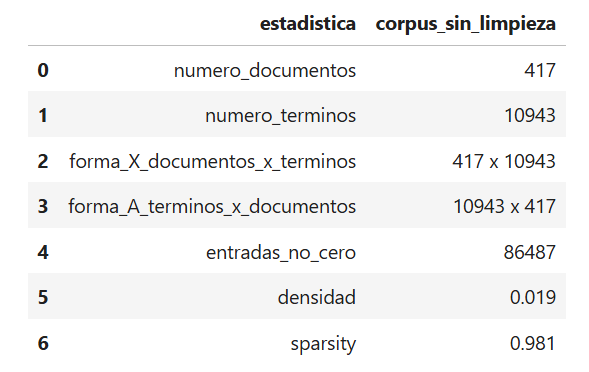
\includegraphics[width=0.5\linewidth]{info.png}
    \label{fig:placeholder}
\end{figure}
\begin{figure}[H]
    \centering
    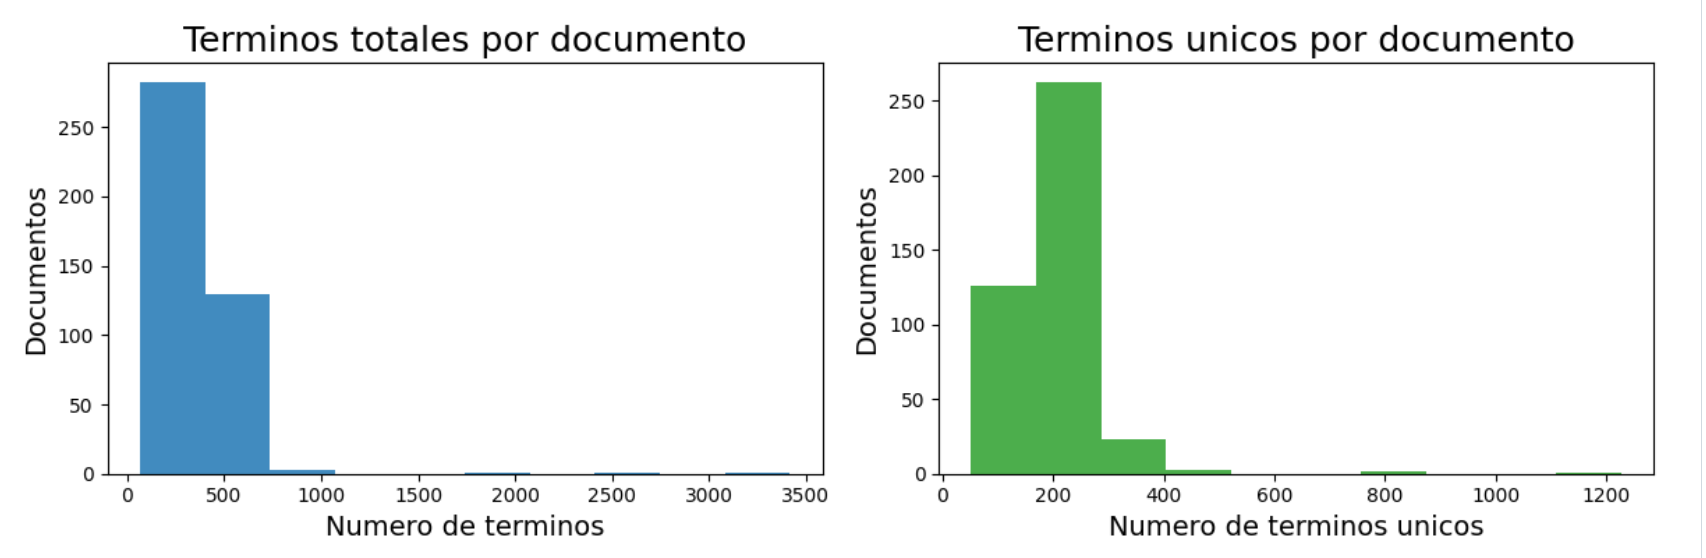
\includegraphics[width=1\linewidth]{grafica.png}
    \label{fig:placeholder}
\end{figure}
Este carpus es interesante por el hecho de comprender que significado semantico latente tenia el Reino Unido en una disputa electoral mas grande en sus ultimos tiempo.

\vspace{0.5cm}

\noindent \textbf{Hipotesis inicial:}

\vspace{0.2cm}

Nuestra hipótesis es que el ambito de política estará dominado por términos como "primer ministro", "lord", "seguridad", "elección", "economía" y "guerra". Dado el contexto del Reino Unido en $2004-2005$, predecimos que los primeros vectores singulares estarán fuertemente alineados con el proceso electoral y la Guerra de Irak.

\vspace{0.2cm}

En el espacio semántico latente, anticipamos una separación entre el poder ejecutivo y el judicial, situando al poder legislativo en una posición intermedia por la division parlamentaria de Reino Unido.

\vspace{0.5cm}

\noindent \textbf{Preprocesamiento de Texto:}
\vspace{0.2cm}

Primero creamos nuestra lista de \textit{stopwords} que es una unión entre las \texttt{ENGLISH\_STOP\_WORDS} de \texttt{sklearn} y \texttt{stop\_words\_custom} (una lista de algunas palabras que decidimos agregar). A esta lista la lematizamos con el modelo \texttt{"en\_core\_web\_sm"} de \texttt{nlp} de la librería \texttt{spacy}.
\vspace{0.2cm}

Creamos una lista (\texttt{documentos\_lem}) con todos los documentos de las noticias, a esta lista le aplicamos igual la lematización de \texttt{spacy}. Luego, creamos nuestra matriz TF-IDF, la cual asigna un puntaje de importancia a cada palabra, el filtro para la creación es de palabras que no esten en los \textit{stopwords} seleccionados, que aparecen en más de $4$ documentos y al menos en el $80$\% de ellos (escogimos este filtro ya que estamos trabajando con más de $400$ documentos), de unigramas y bigramas, estos filtros estrictos nos permiten obtener las palabras que más aportan información y descartar las que no.
\vspace{0.2cm}

Luego, Obtenemos nuestro vocabulario de $4558$ y creamos nuestra matriz término-documento ($A\_final$). Luego creamos un vectorizador para poder obtener el conteo de las palabras y obtenemos nuestro array con la frecuencia de las palabras.

\begin{figure}[H]
    \centering
    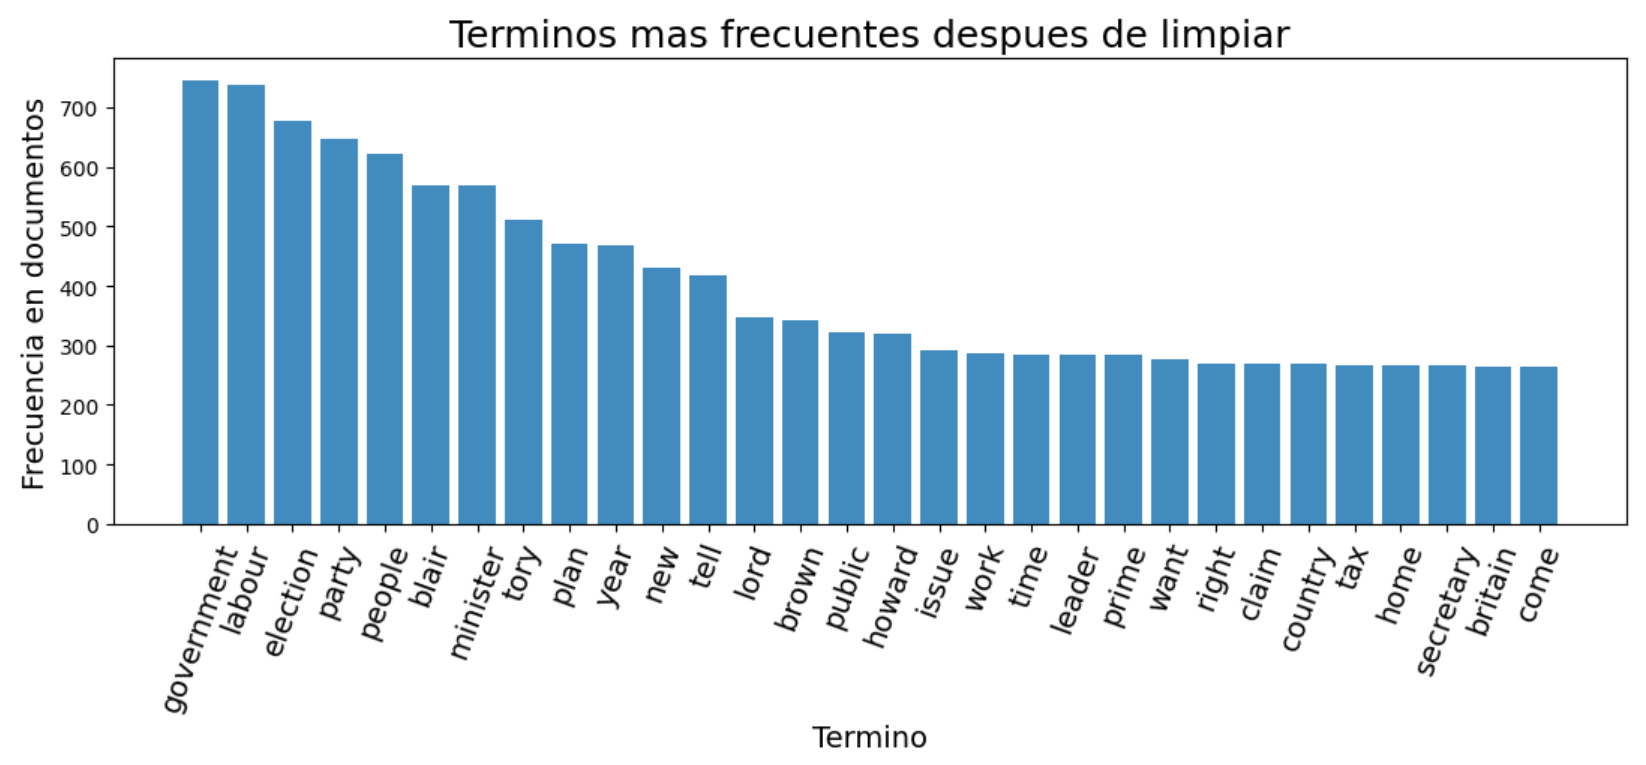
\includegraphics[width=1\linewidth]{grafico_2.png}
    \label{fig:placeholder}
\end{figure}
\noindent \textbf{Construccion de la matriz textual:}
\vspace{0.2cm}

Utilizamos \textit{scikit-learn} que entrega una matriz con documentes en las filas y términos en las columnas por lo tanto obtenemos su transpuesta para poder trabajo con la matriz con términos en las filas y documentes en las columnas.

\vspace{0.2cm}

La matriz resultante es la siguiente:
\begin{itemize}
    \item \textbf{Dimensiones (términos $\times$ documentos):} $(4558, 417)$.
    \item \textbf{Representación de componentes:} Una entrada $A_{ij}$ representa el puntaje TF-IDF (Frecuencia de Término - Frecuencia Inversa de Documento) del término $i$ en el documento $j$. Este valor numérico indica qué tan importante o relevante es el término $i$ específicamente para el documento $j$
\end{itemize}
\vspace{0.5cm}

\noindent \textbf{Calculo de la SVD:}
\vspace{0.2cm}

Los valores singulares representan la cantidad de información(varianza) que captura cada tema, el primer valor es el más dominante, en cambio los últimos son temas raros. Los vectores singulares izquierdos representan la relación de las palabras con los temas y los vectores derechos representan la relación de los temas con los documentos.

\vspace{0.5cm}

\noindent \textbf{Valores singulares y eleccion de dimension:}
\vspace{0.2cm}

Veamos la grafica de los 3 primeros valores singulares:
\begin{figure}[H]
    \centering
    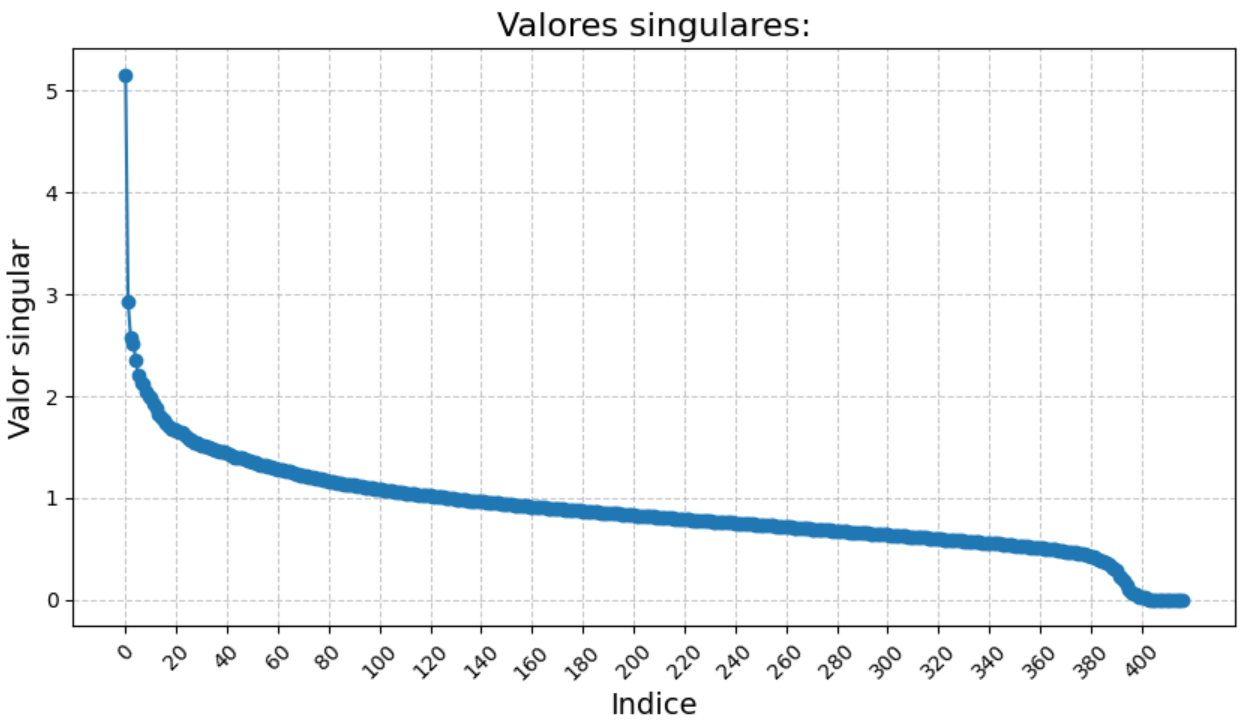
\includegraphics[width=1\linewidth]{grafica_3.png}
    \label{fig:placeholder}
\end{figure}
Se observa una caída pronunciada al inicio. Elegimos $k =22$ basándonos en el método del codo, ya que a partir de este componente la magnitud de los valores singulares se estabiliza, indicando que el resto de las componentes representan mayoritariamente ruido en lugar de estructura semántica relevante del corpus.

\vspace{0.5cm}

\noindent \textbf{Representacion de documentos y terminos en baja dimension:}
\vspace{0.2cm}

Veamos los primeros 3 valores singulares.

\begin{figure}[H]
    \centering
    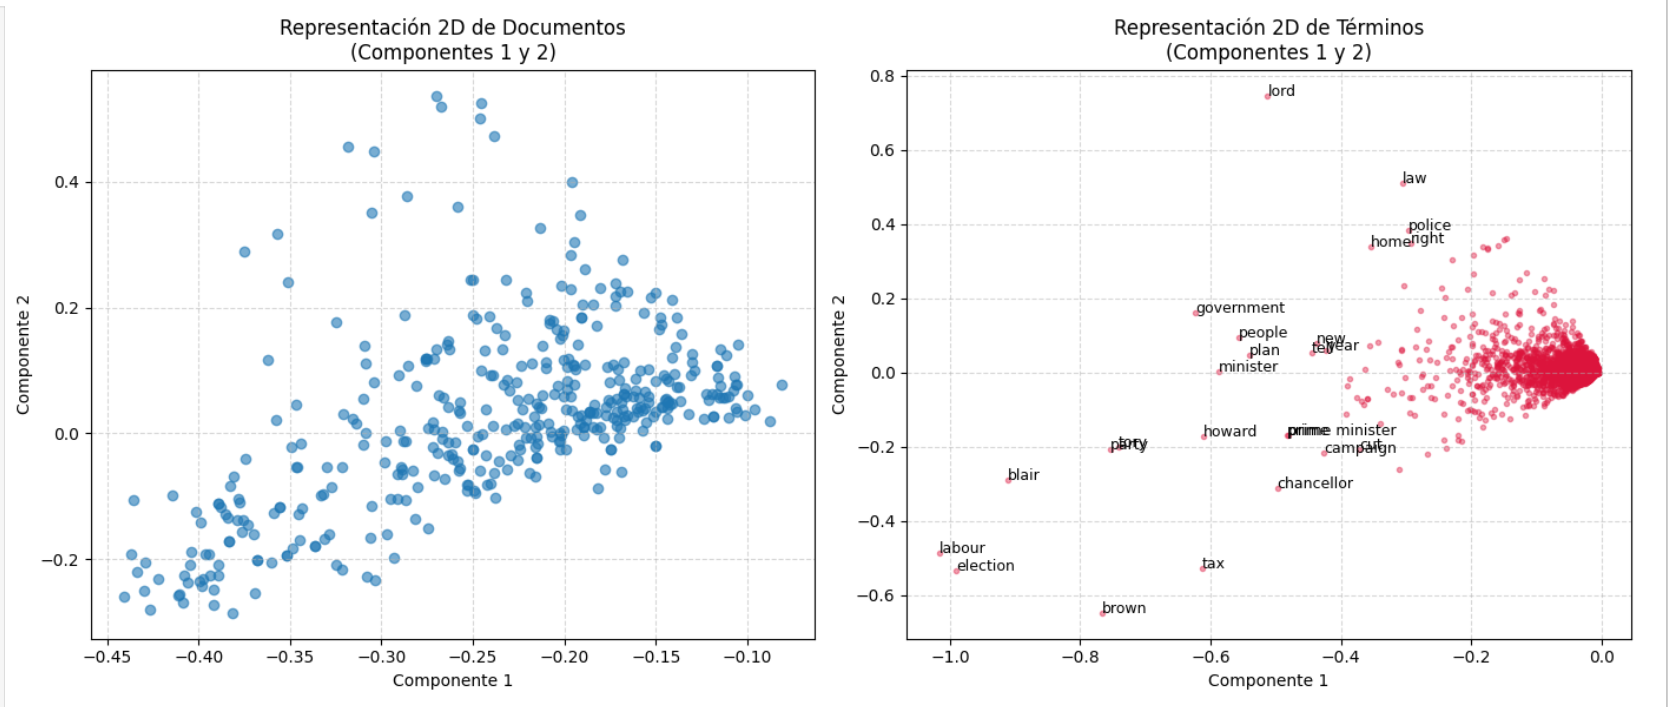
\includegraphics[width=1.1\linewidth]{grafico_componente_1.png}
    \caption{Grafico componente 1}
    \label{fig:placeholder}
\end{figure}

\begin{figure}[H]
    \centering
    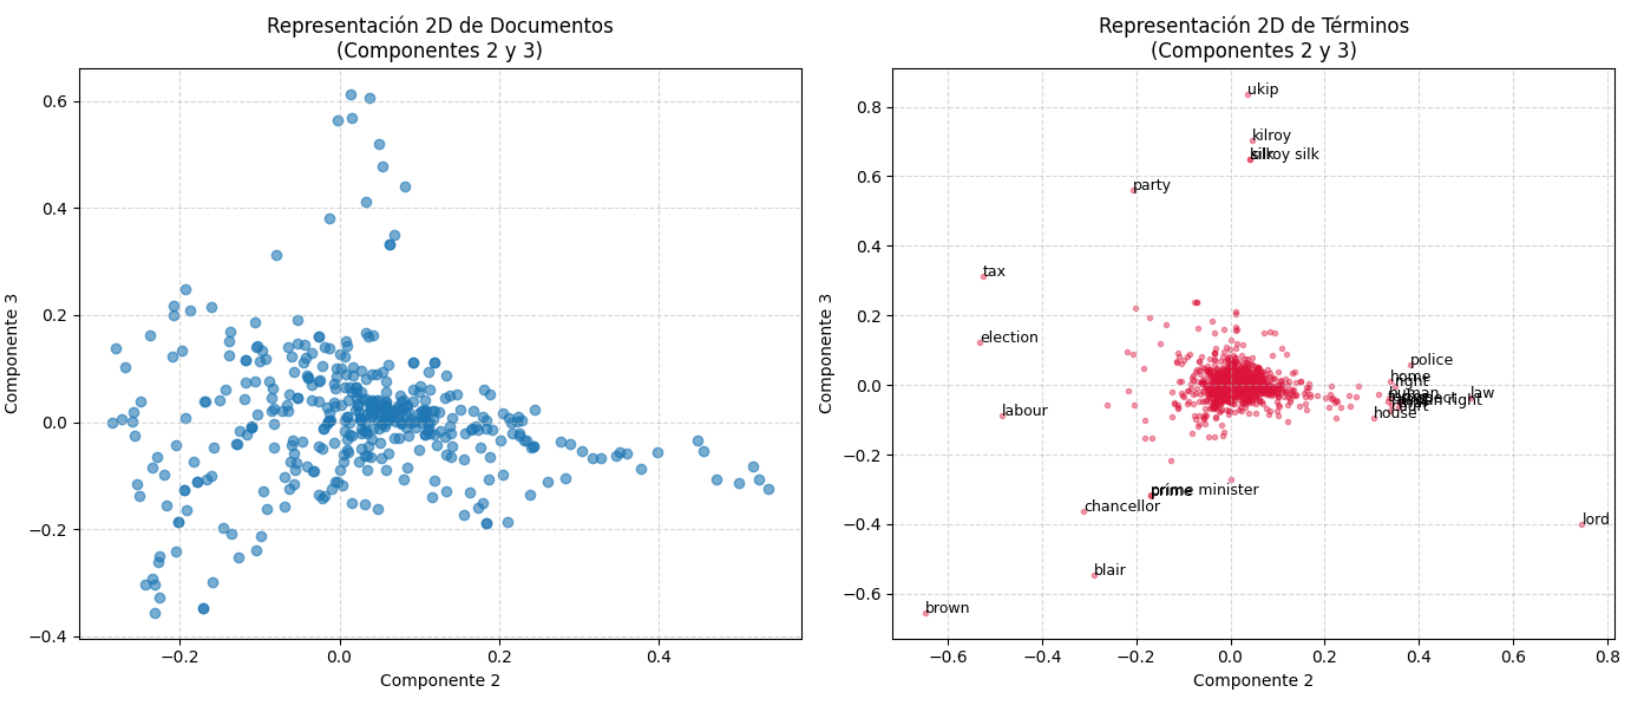
\includegraphics[width=1.1\linewidth]{grafico_componente_2.png}
    \caption{Grafico componente 2}
    \label{fig:placeholder}
\end{figure}
Analizamos las 3 principales dimensiones:

\begin{itemize}
    \item \textbf{Componente 1:} Representa la pelea electoral del Reino Unido durante el año 2005. Hacia el valor $-1$, se observan los elementos que constituyen directamente la pelea electoral teniendo a blair (Actual primer ministro) vs howard (Su principal competencia), en cambio, hacia el valor $0$, se encuentran los elementos que están indirectamente relacionados con dicha disputa. Al notar que no tenemos valores positivos, podemos concluir que no hay un tema que rivalice directamente con la pelea electoral, lo que convierte a este conflicto en el eje central de toda la información.
    \item \textbf{Componente 2:} 
Representa la separación entre el Poder Judicial y la política de seguridad en el valor $1$, asociado a los lord, leyes y policia. Frente a la política económica en el valor $-1$. Esta última se asocia específicamente a la figura de Brown (Ministro de Hacienda) y al impuestos (tax). En el centro del eje se ubica el Poder Legislativo.
    \item \textbf{Componente 3:}
Representa la separacion hacia los valores $1$ los partidos politicos (ukip) o relacionado y al otro extremo en el valor $-1$ las palabras mas alto del gobierno como (lord, blair), vemos en el centro el partido actual del gobierno (labour) que representa ambos lados y palabras como policia y casas que no tiene conexcion con los valores de los extremos.

\end{itemize}


\vspace{0.5cm}

\noindent \textbf{Exploracion semantica:}
\vspace{0.2cm}

\vspace{0.5cm}

\noindent \textbf{Discusion, limitaciones y conclusiones:}
\vspace{0.2cm}

Viendo los graficos de componentes 1 y 2 veamos que palabras dominar. Dominaron nombres de políticos (Brown, Blair, Howard, Kilroy) y partidos (Labour, UKIP). Los temas (elecciones, impuestos, leyes, ministros) coincidieron con la hipótesis, aunque se omitieron nombres de partidos y la figura fundamental de los Lords en el ámbito judicial y legislativo.
\vspace{0.2cm}

Se hallaron dos omisiones relevantes o un componente muy lejano: la Reina Isabel II, reflejando su rol neutral y simbólico, y la Guerra de Irak, pese a ser una crítica central al mandato de Blair.

\begin{figure}[H]
    \centering
    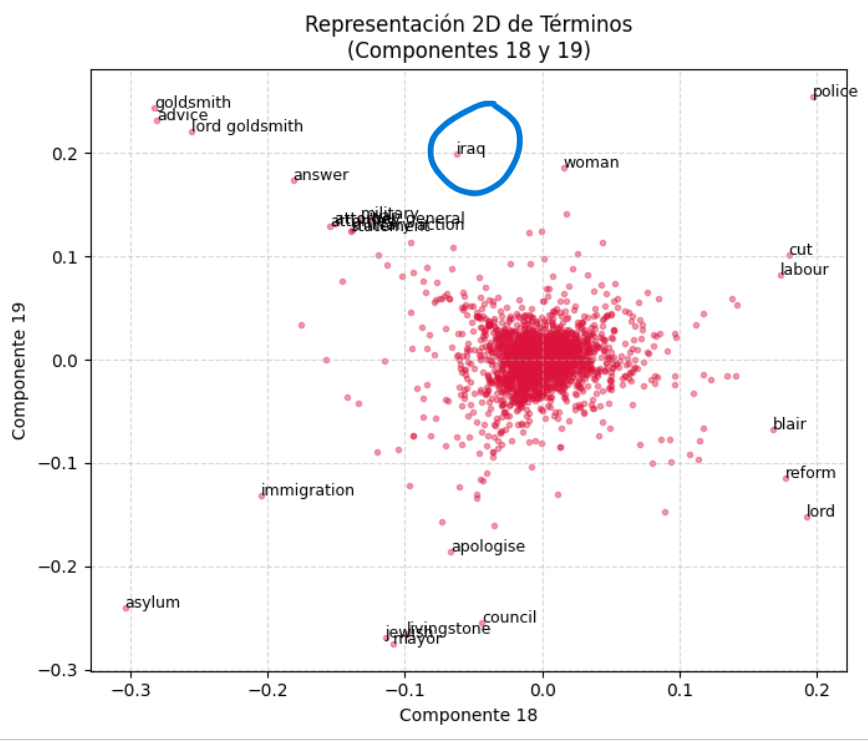
\includegraphics[width=1\linewidth]{grafico_componente_5.png}
    \label{fig:placeholder}
\end{figure}
\vspace{0.2cm}

Los vectores singulares muestran un eje principal centrado en el proceso electoral veamos el grafico componente 2. El eje X confirma nuestra hipótesis: la división del Parlamento en tres bloques. El Ejecutivo (Ministro) y el Judicial (Lords) en los extremos, con el Legislativo (Cámara de los Comunes) al centro como espacio de debate partidista y ministros, donde las leyes transitan hacia la aprobación de los Lords.
\vspace{0.2cm}

Encuentro unas de las limitaciones que se centra puramente en la inpretracion de los temas, que te pide un manejo bastante bueno para un buen analisis, como ejemplo resalta mas los nombres de los politicos mas que sus cargos. Otro limitacion seria que es en base a datos de palabras en este caso a noticia, por lo cual el analisis siempre va a estar con la frase en "base a la noticia" como en La Guerra de Irak que si paso y fue unos de los temas politico importate auque en la LSA de la noticia no lo coloca como los principales.
\vspace{0.2cm}

En conclusion la LSA es un buena herramienta para comprender, explorar sobre un carpus y como se relaciona sus terminos, pero necesario un solido conocimiento del tema, y ademas queda la LSA con el sesgo de la fuente.
\vspace{0.5cm}
 
\begin{thebibliography}{9}

\bibitem{terry-dataset}
\noindent Terry, A. F. (s.f.). \textit{BBC News Dataset (Clean CSV Version)}. Kaggle. Recuperado de: \url{https://www.kaggle.com/datasets/alfathterry/bbc-full-text-document-classification}

\bibitem{github} 
Gutiérrez, N. y Zambrano, D. (2026). \textit{Algoritmos de SVD y visualización de datos para análisis LSA}. Repositorio de GitHub: \url{https://github.com/Skysilen-t/Proyecto-1-LSA-con-SVD/tree/main}
\smallskip


\end{thebibliography}
\end{document}
